\ \\
\linebreak
Wie können wir uns das formale Konstrukt $\div F$ 
anschaulich vorstellen? Setzen wir zum Beispiel $F$ als 
Geschwindigkeitsfeld einer strömenden Flüssigkeit an, so können 
wir  
\begin{equation*}
	\int_{\partial Q}F\cdot r \ \mathrm{d}a
\end{equation*}
als ein Maß für den Massentransport (pro Zeiteinheit) durch 
die Oberfläche eines Quaders $Q$ ansehen. Ist der (skalierte) 
Mittelwert dieses Flusses 
\begin{equation*}
	\frac{1}{v_n(Q)}\int_{\partial Q}F\cdot r \ \mathrm{d}a
\end{equation*}
positiv, so spricht man anschaulich von einem ''Zufluss'' und analog dazu, falls er negativ ist, von einem ''Abfluss''. Ist 
er gleich Null, so handelt es sich um eine ausgeglichene Bilanz.

\begin{lemma}
Sei $F:U\subset\mathbb{R}^n\rightarrow\mathbb{R}$ ein stetig 
differenzierbares Vektorfeld und $U$ offen. Dann sei weiter 
$\tilde{x}\in U$ und $\{Q_k\}$ eine Folge von Quadern, deren 
Abschluss $\overline{Q}$ Teilmenge von $U$ ist, sodass 
$\tilde{x}\in Q_k \ \forall k$. Außerdem soll $r_k>0$ als 
größte Kantenlänge von $Q_k$ für $k\rightarrow\infty$ gegen Null 
gehen. Dann gilt
\begin{equation}
	\lim\limits_{k\rightarrow\infty}\frac{1}{v_n(Q)}\int_{\partial Q} F\cdot r\ \mathrm{d}a = 
	\mathrm{div\ }F(\tilde{x})
\end{equation} 
\end{lemma}

\begin{proof}
Da alle $\overline{Q}_k$ kompakt sind und $\mathrm{div\ }F$ stetig ist, existiert ein $a_k\coloneqq\min\limits_{x\in\overline{Q}_k}\mathrm{div\ }F(x)$ und ein $b_k\coloneqq\max\limits_{x\in\overline{Q}_k}\mathrm{div\ }F(x)$, so dass 
wir nach Satz 31.2 folgern können
\begin{equation*}
	a_k\cdot v_n(Q)\leq\int_{Q_k}\mathrm{div\ }F(x)\mathrm{d}x 	= \int_{\partial Q_k}F\cdot r \ \mathrm{d}a \leq 
	b_k\cdot v_n(Q_k)
 \end{equation*}
Aus 
\begin{equation*}
	\lim\limits_{k\rightarrow\infty} a_k = 
	\lim\limits_{k\rightarrow\infty} b_k = 
	\mathrm{div\ }F(\tilde{x})
\end{equation*}
folgt dann die Behauptung.
\end{proof}
\ \\
\linebreak
Somit nennt man einen Punkt $x$ \textbf{Quelle} von $F$, falls 
$\mathrm{div\ }F(x)>0$ und \textbf{Senke}, falls $\mathrm{div\ }F(x)<0$. Die Divergenz $\mathrm{div\ }F$ können wir dann 
schließlich auch als Quellendichte von $F$ bezeichnen. (32.5) 
besagt somit, dass die Summe der in $Q$ erzeugten 
beziehungsweise vernichteten Flüssigkeit durch den Rand des 
Quaders ab- oder zufließen muss. Dieser Gedanke für auf viele 
grundlegende Bilanzgleichungen der Physik. 
\newpage
\begin{theorem}[Gaußscher Integralsatz]
Sei $\Omega\subset\mathbb{R}^n$ offen, beschränkt und habe 
einen stückweise glatten Rand. Außerdem sei $F:\overline{\Omega} 
\rightarrow\mathbb{R}^n$ stetig und differenzierbar auf $\Omega$ und sei $\mathrm{div\ }F$ integrierbar auf $\Omega$. 
Dann gilt
\begin{equation}
	\int_\Omega\mathrm{div\ }F(x)\mathrm{d}x = 
	\int_{\partial\Omega}F(x)\cdot\nu(x)\ \mathrm{d}a
\end{equation}
\end{theorem}
\ \\
Hierbei ist zu bemerken, dass $F:U\rightarrow\mathbb{R}^n$, 
falls es stetig differenzierbar auf der offenen Umgebung $U$ 
von $\overline{\Omega}$ ist, schon alle Bedingungen für 
Theorem 32.4 erfüllt. \\
Außerdem bleibt anzumerken, dass der Gaußsche Integralsatz 
auch richtig bleibt, wenn $\Omega$ einen Lipschitz-Rand hat, 
der sich als Graph einer Lipschitz-stetigen Funktion 
darstellen lässt.\\
\linebreak

\emph{Beweisstrategie:} Man zeigt die Behauptung zunächst 
für ein $F$ mit kompaktem Träger.\\
\linebreak

Gelegentlich wird der Gaußsche Satz auch in folgender Form definiert:

\begin{satz}[Variante des Gaußschen Satzes]
Sei $\Omega\subset\mathbb{R}^n$ offen, beschränkt und habe 
einen stückweise glatten Rand. Außerdem sei $f:\overline{\Omega}\rightarrow\mathbb{R}$ als skalare 
Funktion stetig und differenzierbar auf $\Omega$ und 
$\pdiff{}{x_n}f$ integrierbar auf $\Omega$. 
Dann gilt
\begin{equation}
	\int_\Omega\pdiff{}{x_k}f(x)\mathrm{d}x = 
	\int_{\partial\Omega}f(x)\cdot\nu_k(x)\ \mathrm{d}a
\end{equation}
wobei $\nu_k$ die k-te Komponente des Einheitsnormalenfeldes 
$\nu$ ist.
\end{satz}

\begin{proof}
Wir definieren das Vektorfeld $F(x)\coloneqq 
(0,0,. . .,f_k(x),. . .,0)$, welches alle Voraussetzungen 
für Theorem 32.4 erfüllt. Damit impliziert (32.8) gerade 
(32.9).
\end{proof}
\ \\
Es fällt auf, dass wir auch Satz 32.5 als eigentlich Satz 
von Gauß hätten formulieren können, denn mit $F = 
(F^1,...,F^n)$ erfüllen alle $f=F^k$ die Voraussetzungen 
für Satz 32.5. Dann summieren wir einfach alle $\int_\Omega F_{x_k}^k\mathrm{d}x$ auf und erhalten (32.8).

\begin{theorem}[Partielle Integration]
Sei $\Omega\subset\mathbb{R}^n$ offen, beschränkt und mit 
stückweise glattem Rand, dann gilt
\begin{enumerate}
	\item 	Sind $f,g:\overline{\Omega}\rightarrow\mathbb{R}$ 
			stetig und stetig differenzierbar auf 
			$\Omega$ und $f_{x_k},g_{x_k}$ integrierbar auf 
			$\Omega$, dann 
			\begin{equation}
				\int_\Omega f_{x_k}(x)g(x)\mathrm{d}x = 
				- \int_\Omega f(x)g_{x_k}(x)\mathrm{d}x + 
				\int_{\partial\Omega}f(x)g(x)\nu_k(x)\mathrm{d}a
			\end{equation}
	\item Sind $F:\overline{\Omega}\rightarrow\mathbb{R}^n$ 
			und $g:\overline{\Omega}\rightarrow\mathbb{R}$ 
			jeweils stetig und stetig differenzierbar auf 
			$\Omega$, sowie div $F$ und $g'$ integrierbar 
			auf $\Omega$, dann
			\begin{equation}
				\int_\Omega F(x)g'(x)\mathrm{d}x = 
				-\int_\Omega g(x)\mathrm{div\ }F(x)\mathrm{d}x + 
				\int_{\partial\Omega}g(x)F(x)\nu(x)\mathrm{d}a
			\end{equation}
\end{enumerate}
\end{theorem}

\begin{proof}
Für 1. wenden wir (32.8) auf $f\cdot g$ an und erhalten die 
Behauptung. Für 2. wenden wir (32.8) auf das Vektorfeld 
$g\cdot F$ an. Dabei ist zu beachten, dass
\begin{equation*}
	\mathrm{div\ }(gF)=g\cdot\mathrm{div\ }F + F\cdot g'
\end{equation*}
\end{proof}
\ \\
Gerade in der Potentialtheorie ($\Delta\varphi=f$) sind folgende 
Formeln wichtig:
\newpage
\begin{satz}[Greensche Formeln]
Sei $\Omega\subset\mathbb{R}^n$ offen, beschränkt und mit 
stückweise glattem Rand. Außerdem seien $f,g:\overline{\Omega} 
\rightarrow\mathbb{R}$ stetig und in $C^2$ auf $\Omega$, 
dann gilt, falls die Integrale existieren, folgendes:
\begin{equation}
	\int_\Omega f'(x)\cdot g'(x)\mathrm{d}x = 
	-\int_\Omega f(x)\Delta g(x)\mathrm{d}x + 
	\int_{\partial\Omega}f(x)g'(x)\nu(x)\mathrm{d}a
\end{equation}
\begin{equation}
	\int_{\Omega}f(x)\Delta g(x)-g(x)\Delta f(x)\mathrm{d}x = 
	\int_{\partial\Omega}f(x)g'(x)\nu(x) - 
	g(x)f'(x)\nu(x)\mathrm{d}a 
\end{equation}
wobei $\Delta f(x)=\mathrm{div\ }f'(x)$.
\end{satz}

\begin{proof}
Wir verwenden (32.11) mit ($g',f$) statt ($F,G$) und kommen 
damit auf (32.12) mit ($f,g$) und ($g,f$) und erhalten damit
(32.13).
\end{proof}

\begin{beispiel}
Sei $\Omega\subset\mathrm{R}^n$ wie in Theorem 32.4 und $F(x) = 
x$. Offenbar ist $\mathrm{div\ }F(x)=n$ auf $\Omega$, daraus 
folgt mit (32.8)
\begin{equation}
	nv_n(\Omega)=\int_{\partial\Omega}x\cdot\nu(x)\mathrm{d}a
\end{equation}
\begin{enumerate}
	\item  $\Omega=B_1(0)$. Hier ist $x\cdot\nu(x)=1$ auf
			$\partial\Omega$ und nach (32.14) gilt dann
			\begin{equation*}
				n\kappa_n=\omega_n
			\end{equation*}
			\begin{center}
				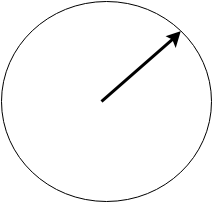
\includegraphics[scale=0.5]{pictures/008-01.png}				\end{center}			 
\newpage
	\item $\Omega\subset\mathbb{R}^2$. Hier sei der Rand eine 
			$C^2$-Kurve $t\rightarrow(x(t),y(t))$ dann ist
			\begin{equation*}
				\nu(x(t),y(t)) =
				\frac{(y'(t),-x'(t)}{|(y'(t),-x'(t)|}
			\end{equation*}
			Daraus folgt mit (32.14)
			\begin{equation*}
				v_2(\Omega) = 
				\frac{1}{2}\int\limits_a^b\frac{xy'-yx'}
				{\sqrt{x'^2+y'^2}}\sqrt{x'^2+y'^2}\mathrm{d}t = 
				\frac{1}{2}\int\limits_a^bx(t)y'(t)-y(t)x'(t) \ 
				\mathrm{d}t
			\end{equation*}
			\begin{center}
				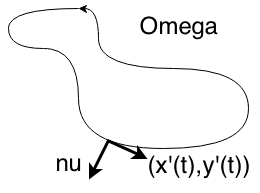
\includegraphics[scale=0.5]{pictures/008-02.png}\end{center}	
\end{enumerate}
\end{beispiel}

Nach dem Satz von Gauß kommen wir nun zu einem zweiten wichtigen Integralsatz, dem Satz von Stokes. Dazu klären wir zunächst ein 
paar Begriffe.
\begin{definition}[Rotation]
Sei $F:\Omega\subset\mathbb{R}^3\rightarrow\mathbb{R}^n$ ein 
$C^1$-Vektorfeld auf dem offenen $\Omega$ mit $F=(F^1,F^2,F^3)$. 
Das Vektorfeld $\rot F:\Omega\rightarrow\mathbb{R}^n$ 
gegeben durch
\begin{equation}
	\rot F(x)\coloneqq 
	\begin{pmatrix}
	\pdiff{}{x_2}F^3(x)-\pdiff{}{x_3}F^2(x) \\
	\pdiff{}{x_3}F^1(x)-\pdiff{}{x_1}F^3(x) \\
	\pdiff{}{x_1}F^2(x)-\pdiff{}{x_2}F^1(x)
	\end{pmatrix}
\end{equation}
heißt \textbf{Rotation} oder auch Zirkulation von $F$. Sie 
lässt sich auch sehr effektiv durch den \textbf{Nabla-Operator} 
gewinnen. 
\begin{equation*}
	\nabla\coloneqq e_1\pdiff{}{x_1}+e_2\pdiff{}{x_2} + 
	e_3\pdiff{}{x_3}
\end{equation*}
\begin{equation*}
	\rot F=\nabla\times F=\det\begin{pmatrix}
	e_1 & e_2 & e_3 \\
	\pdiff{}{x_1} & \pdiff{}{x_2} & \pdiff{}{x_3} \\
	F^1 & F^2 & F^3  
	\end{pmatrix}
	\tag{32.15'}
\end{equation*}
\end{definition}

\begin{beispiel}
Betrachten wir das Vektorfeld 
\begin{equation*}
	F(x)\coloneqq \begin{pmatrix}
	0 \\ 0 \\ \alpha \end{pmatrix} \times
	\begin{pmatrix}
	x_1 \\ x_2 \\ x_3 \end{pmatrix} = 
	\begin{pmatrix}
	-\alpha x_2 \\ \alpha x_1 \\ 0 \end{pmatrix} 
\end{equation*}
Aufgrund des Kreuzproduktes steht $F(x)$ immer senkrecht auf $x$ . Die Rotation ist
\begin{equation*}
	\rot F(x) = \begin{pmatrix}
	0 \\ 0 \\ 2\alpha
	\end{pmatrix}
\end{equation*}
Wir können das ganze so interpretieren, dass $F(x)$, falls die Rotation nicht verschwindet, nahe $x$ um die Achse 
\begin{equation*}
	\left\{ x + t\cdot\rot F(x)\middle| 
	t\in\mathbb{R}\right\}
\end{equation*}
\emph{rotiert}, wobei $|\rot F(x)|$ ein Maß für die 
\emph{Rotationsgeschwindigkeit} ist. Ist diese ungleich Null, so sagt man, dass $F$ einen Wirbel in $x$ hat.
\end{beispiel}

\begin{satz}[Rechenregeln]
Seien $F,G:\Omega\subset\mathbb{R}^3\rightarrow\mathbb{R}^3$ 
beides $C^1$-Vektorfelder auf dem offenen $\Omega$ und 
$g:\Omega\rightarrow\mathbb{R}$ ebenfalls $C^1$. Dann gilt
\begin{enumerate}
	\item 	Linearität
			\begin{equation*}
				\rot (\alpha F + \beta G) = 
				\alpha\rot F + \beta\rot G
			\end{equation*}
	\item 	Produktregel
			\begin{equation*}
				\rot (gF)=g\rot F+g'\times F
			\end{equation*}
	\item 	Gradienten sind wirbelfrei.
			\begin{equation*}
				\rot g' = 
				\rot \grad g=0
			\end{equation*}
	\item 	Rotationsfelder sind quellenfrei.
			\begin{equation*}
				\div \rot  F = 0
			\end{equation*}
\end{enumerate}
\end{satz}
\begin{proof}
Lässt sich mit (32.15) oder (32.15') leicht nachrechnen.
\end{proof}